\appendix
\section{附录}

\subsection{缩略语对照表}

\begin{table}[H]
  \centering
  \caption{缩略语}
  \label{tab:abbrev}
  \begin{tabularx}{0.6\textwidth}{p{2.5cm}|X}
    \toprule
    \textbf{缩略语} & \textbf{全称} \\
    \midrule
    GIS   & Geographic Information System \\
    POI   & Point of Interest \\
    API   & Application Programming Interface \\
    CRUD  & Create, Read, Update, Delete \\
    MVP   & Minimum Viable Product \\
    \bottomrule
  \end{tabularx}
\end{table}

\subsection{参考文献}

（待填写：高德地图 API 文档、FastAPI 官方文档、Vue 3 文档等。）

\subsection{项目仓库}

（待填写：GitHub 仓库地址、分支说明。）

\subsection{页面截图}

页面截图已统一放置在 \texttt{figures/} 目录，正文第 7 章按功能模块引用主要页面截图。

\begin{figure}[H]
  \centering
  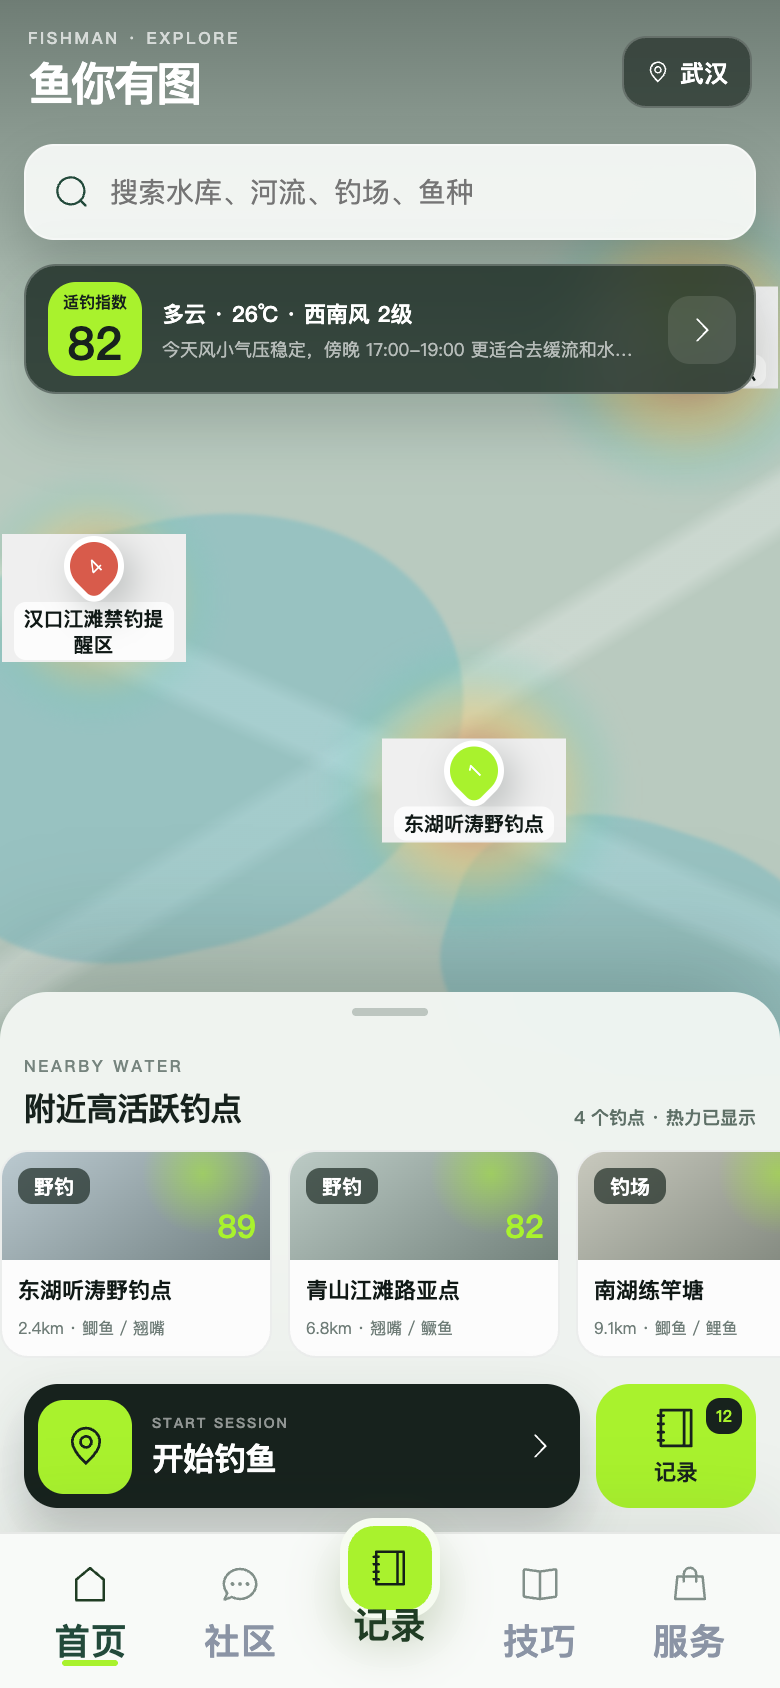
\includegraphics[height=0.68\textheight]{figures/page_home.png}
  \caption{首页截图（示例）}
  \label{fig:appendix-page-home}
\end{figure}
